%!TEX root = ../main.tex
%%%%%%%%%%%%%%%%%%%%%%%%%%%%%%%%%%
% Links: https://leetcode.com/problems/find-minimum-in-rotated-sorted-array/
%
% Difficulty: Medium
% Companies: 
%%%%%%%%%%%%%%%%%%%%%%%%%%%%%%%%%%

\chapter{Minimum element in rotated sorted array}
\label{ch:min_rotated_array}
\section*{Introduction}
In this chapter, we will tackle a very popular interview question that has a surprisingly short statement and an obvious linear time solution. However, solving this problem nicely is a different story, and coming up with an elegant and efficient solution requires a fair amount of thinking and careful coding.

This problem is based upon the concept of array rotations. To develop an intuitive understanding of this concept, imagine that we want to "rotate" the elements of an array, that is to shift all of them to the right by a certain number $k$ of positions. The element that was used to be at position $0$ is now at position $k$ and the element that was at position one is now at $k+1$ and so on (see Figure \ref{fig:min_rotated_array:arrayrotation} for an example).

\begin{figure}
	\centering
	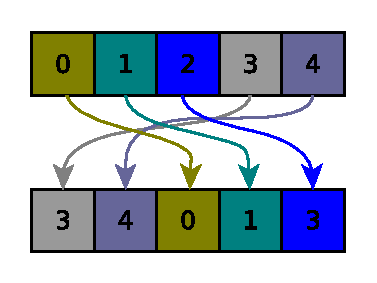
\includegraphics{sources/min_rotated_array/images/arrayrotation}
	\caption{Example of array rotation where every element if moved to the right of 2 positions. Notice how elements at position $3$ and $4$ are wrapped around to positions $1$ and $2$, respectively.}
	\label{fig:min_rotated_array:arrayrotation}
\end{figure}


\section{Problem statement}
\begin{exercise}
Given an array $A$ sorted in ascending order with no duplicates and rotated around a pivot, return the smallest element.

	\begin{example}
		\hfill \\
		Given the rotated array $\{3,4,5,6,1,2\}$ the function returns $1$.
	\end{example}

	\begin{example}
		\hfill \\
		Given the rotated array $\{0,2,3\}$ the function returns $0$.
	\end{example}

	\begin{example}
		\hfill \\
		Given the rotated array $\{3,2,1\}$ the function returns $1$.
	\end{example}
\end{exercise}

\section{Clarification Questions}

\begin{QandA}
	\item Are all the elements unique? 
	\begin{answered}
		\textit{Yes, you can assume all the elements are unique}
	\end{answered}
	\item Can the input array be empty?
	\begin{answered}
		\textit{No, you might assume the array contains at least one element.}
	\end{answered}
\end{QandA}

\section{Discussion}
\label{min_rotated_array:sec:discussion}
What does it really mean for a sorted array to be rotated around an element? Given a sorted array $A=\{a_0, a_1, \ldots,a_{n-1}\}$ s.t. $ \forall \: 0 \leq i < n: a_i < a_{i+1}$, rotating A around the pivot element at index $p$ results in: $A_p=\{a_p, a_{p+1}, \ldots,a_{n-1}, a_0, a_1, \ldots, a_{p-1}\}$. In a nutshell all the elements are rotated in such a way that the element at index $p$ becomes the first element of the array. For instance, rotating the array $X=\{1,2,3,4,5\}$ around the element at index $2$, results in $X=\{3,4,5,1,2\}$. We would obtain the same result by applying a offset of either $-2$ or $3=5-2=(|A|-2)$ positions to each and every element of $X$. 

This way of performing rotation is quite common, to the point that there is an algorithm in the C++ STL\cite{cit::std::rotate} adopting such API.

\subsection{Brute-force}
\label{min_rotated_array:sec:bruteforce}
The brute-force solution to this problem is trivial and consists of simply looping through the array and keeping record of the smallest element encountered.
In C++ this can be implemented with a one-liner as shown in Listings \ref{list:min_rotated_array_bf} and \ref{list:min_rotated_array_bf_manual} both having $O(n)$ time $O(1)$ space complexity.

\lstinputlisting[language=c++, caption=Brute force solution using an explicit loop.,label=list:min_rotated_array_bf_manual]{sources/min_rotated_array/min_rotated_array_solution2.cpp}

\lstinputlisting[language=c++, caption=One-liner brute force solution.,label=list:min_rotated_array_bf_manual]{sources/min_rotated_array/min_rotated_array_solution2.cpp}

This approach should just be mentioned during the interview but, no time should be spent in the actual implementation of this idea, as the interviewer is assuming you know how to trivially search for the minimum in an unsorted array. He is clearly looking for a more advanced solution that takes advantage of the fact that the array is sorted (even if provided in a rotated form).
Yes, we did not use the word \textit{unsorted} unknowingly, because the interviewer is clearly looking for a more advanced solution that takes advantage of the fact that the array is sorted (even if provided in a rotated form), and the solutions presented above clearly ignore this fact and would work equally well on a random, unsorted and/or unrotated arrays.

\subsection{Logarithmic solution}
\label{min_rotated_array:sec:log}
As usual, when in a problem statement the word \textit{"sorted"} makes its appearance, the first thought that should cross our mind is \textbf{binary search}see Appendix \ref{sect:appendix:binary_search}). In this problem, we are almost forced to think about binary search as the problem does not only involve a sorted input, but it is also about searching. 

How can we use binary search to actually solve this problem, given the fact we have this weirdly sorted array? 
Firstly, notice that despite the fact that the array is not sorted in a canonical way, it still is very much sorted as there is an index $i$ of the array holding the smallest value from which we could iterate the array forward (and eventually continue from the start when we reach the end) and all we would see is a sorted sequence.

In order to be able to apply binary search effectively to a problem, we need some basic ingredients. In particular, we need to be able to:
\begin{enumerate}
	\item keep track of a range of elements that are currently under examination. Binary search works by cutting off parts of a search range until it becomes empty or a solution is found.  Usually such range is initialized to be the closed interval: $[l=0, r=A.size()-1]$ i.e. the entire array;
	\item analyze the element in the middle of this range;
	\item if the middle element is the one we are looking for we are done;
	\item otherwise, the search proceeds either to the left or to the right or the range. 
\end{enumerate}

The core challenges of this problem lie at steps $2$ and $4$ because we need to be able:
\begin{itemize}
	\item test whether an element is the minimum or not ($2$)
	\item decide how to split the space range into two and whether proceed with the search on the right-hand or on the left-hand side ($4$).
\end{itemize}

\subsubsection{Test if an element is the minimum}

In order to decide whether an element $a_k$ at index $k$ is the minimum, it is useful to look at one property that differentiates it from all the other values in the collection.
The minimum element is the only element s.t. both the elements on its right and left are \textbf{greater} than it (sometimes this element is referred to as an inflection point). 
Another useful property that can be helpful in the identification of the minimum is that the element on its left is always the maximum element of the array (see examples (see examples in the Section \ref{min_rotated_array:sec:discussion} and Figure \ref{fig:min_rotated_array:test_element}).
Thus, whenever $a_{k-1} > a_{k}$ (meaning that $a_k$ is the minimum and $a_{k+1}$ the maximum) or $a_{k} > a_{k+1}$ (meaning that $a_k$ is the maximum element and $a_{k+1}$ the minimum) we can stop and return because we have found the answer.

\begin{figure}
	\centering
	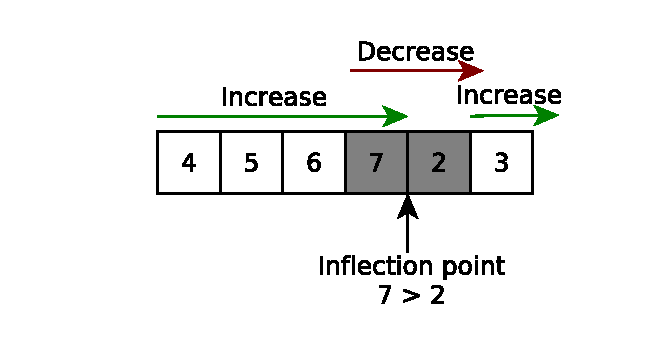
\includegraphics{sources/min_rotated_array/images/inflection_point}
	\caption{Inflection point in a rotated sorted array. When the binary search examines both element $7$ and $2$ it is able to determine the inflection point (element $2$). }
	\label{fig:min_rotated_array:test_element}
\end{figure}

In short, Listing \ref{list:test_answer} shows the condition that can be used in the binary search to test whether $a_k$ is the answer to the problem. Please note how the modulo operation is used in order to avoid having to specialize this test for the elements at the beginning and at the end of the array (positions $0$ and $A.size()-1$, respectively)..

\begin{lstlisting}[language=c++, caption={Test to verify whether the binary search can stop because an answer has been found.},label=list:test_answer]]{
	const int curr = A[k];

	const int prec = A[(k-1+A.size()) 	//+A.size() due to negative modulo
	const int succ = A[(k+1)%A.size()];
	if( (curr <= prec ) || (curr >= succ))
		return min({prec , curr , succ});
}
\end{lstlisting}

\subsubsection{Binary search range split}

The last part of the algorithm yet to be figured out is how and in which split of the array to continue the binary search if the element in the middle of the range is not good to determine the answer. An useful property of the sorted rotated array is that, when the smallest element is at position $i$ then \textbf{all the elements on its right side are smaller than the very first element of the array} (at index $0$) i.e. the following is always true:

\begin{itemize}
	\item $	(a_i < a_0) \: \wedge (a_{i+1} < a_0) \: \wedge \ldots (a_{n-1} < a_0) $
	\item $	(a_{i-1} \geq a_0) \: \wedge \: (a_{i-2} \geq a_0) \: \wedge \: \ldots \: (a_{0} \geq a_0) $
\end{itemize}
For instance, consider the sorted rotated array $\{8,9,10,5,6,7\}$: the minimum element $5$ is at index $3$ and all the elements located between index $3$ and $5$ are strictly smaller than the first element $8$ while all the elements to the left of $5$ are larger or equal than $8$.

This is the last piece of information that is needed in order to make the binary search work, because we can use it to determine which portion of the two subarrays (the one to the left or to the right of \textit{middle}) to discard. Therefore, given an element at position $i$ that is not the answer, we will continue the binary search on the subarray to the left of $i$ if $a_i > a_0$, otherwise we will use the right side.

By being able to test whether an element is the smallest element in the array, and if not, how to split the array and continue the binary search, we have all the ingredients necessary to solve this problem efficiently.

An implementation of this idea is shown in the Listing \ref{list:min_rotated_array_log}.
\lstinputlisting[language=c++, caption={Logarithmic solution implemented using a standard iterative binary search.},label=list:min_rotated_array_log]{sources/min_rotated_array/min_rotated_array_solution3.cpp}


This solution as a complexity of $O(log(n))$ time and $O(1)$ space.
The code is just a straightforward implementation of the binary search where \inline{l} and \inline{r} determine the range under examination, \inline{middle} is the element in the middle of \inline{l} and \inline{r} while \inline{prec} and \inline{succ} are the element preceeding and succeeding \inline{mid}, respectively. Notice how the modulo operation is used to make sure that both \inline{prec} and \inline{succ} always point a valid element. 
